\documentclass{article}
\usepackage[T1]{fontenc}
\usepackage{lmodern}
\usepackage{graphicx}
\usepackage{amsmath,amssymb}
\usepackage[a4paper,margin=2cm]{geometry}
\usepackage[absolute,overlay]{textpos}
\setlength{\TPHorizModule}{1mm}
\setlength{\TPVertModule}{1mm}
\usepackage[indonesian]{babel}
\usepackage{hyperref}
\setlength{\emergencystretch}{2em}
% unit: Halaman 17

\begin{document}

% === Halaman 17 (llm) ===

\vspace{216.81mm}

Contoh penggunaan:

% deskripsi: Screenshot cuplikan kode Python yang menunjukkan contoh penggunaan fungsi xor_cipher_encrypt dan xor_cipher_decrypt, lengkap dengan input pengguna untuk nama file plaintext, ciphertex, dan kata kunci.
% bbox normalisasi: [0.1070, 0.2010, 0.7220, 0.9310]
\begin{textblock*}{129.15mm}(22.47mm,59.70mm)
\noindent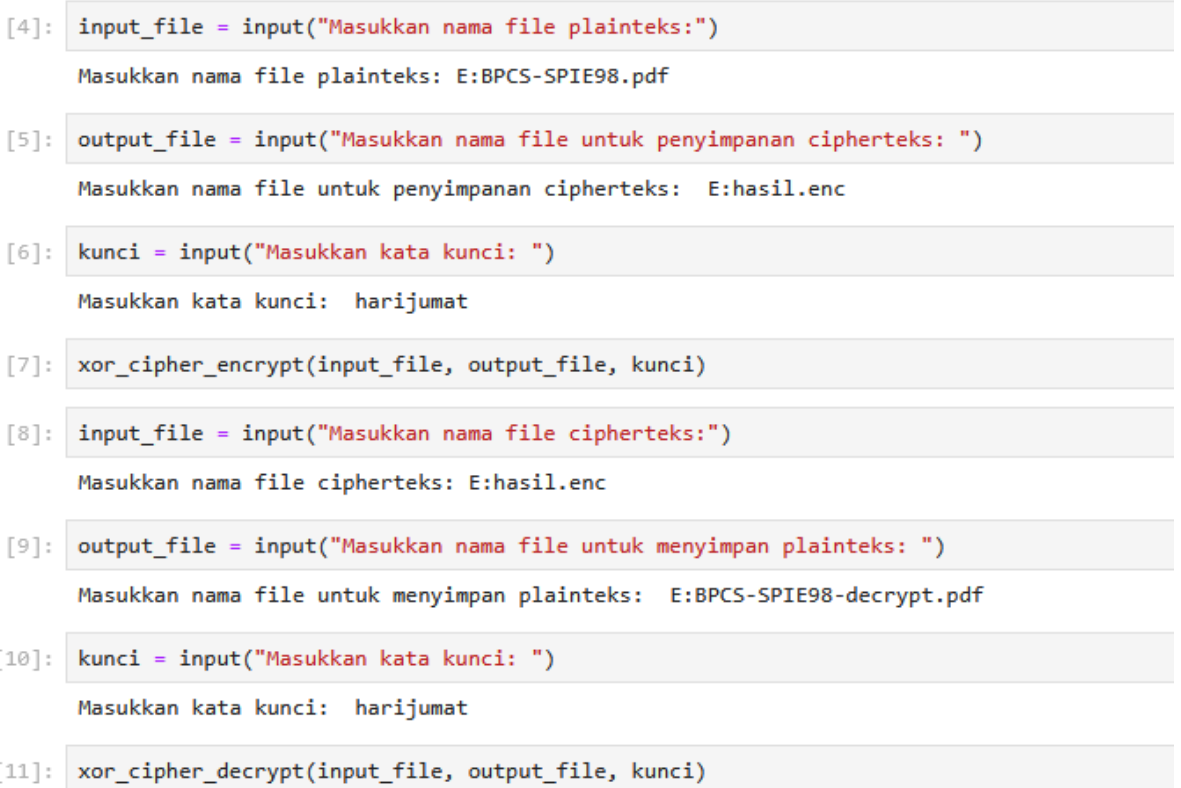
\includegraphics[width=129.15mm,height=216.81mm]{../../images/llm/page_017_img_01.png}%
\end{textblock*}

\end{document}
